\chapter{Interactive Message-Locked Encryption}
\label{chap:imle}

\begin{quote} \small
	This chapter looks at the definition and security for interactive message-locked encryption.
\end{quote}

\noindent
In \cite{imle}, MLE was extended to a new scheme called iMLE. An interactive message-locked encryption scheme ($\mathsf{iMLE}$ is defined by four procedures defined below - one algorithm and three protocols.
\begin{enumerate}
	\item $\mathsf{Init}(\secparam)$ - The initialization algorithm run by the server. This will set up the initial server-side state $\serv$.
	
	\item $\mathsf{Reg}$ - This protocol, initiated by the client will register the client with the server. The server returns client parameters $\client \in \bin^*$ which is output by the protocol.
	
	\item $\mathsf{Put}(M, \client)$ - The put protocol takes as input the plaintext and the client credentials. It stores the file and outputs an identifier $f$. Client genertaes key $K \leftarrow \mathcal{K}_{p}(M)$ and then generates the ciphertext $C \leftarrow \mathcal{E}_{p}(K, M)$. Note that $p$ is the public parameter generated by the $\mathsf{Init}$ procedure.
	
	\item $\mathsf{Get}(f, \client)$ - The get protocol takes as input the client parameters and file identifier and outputs the plaintext $m \in \bin^*$
\end{enumerate}

We follow the notation for protocols as given in \cite{imle}.
\begin{itemize}
	\item A protocol $\mathsf{P}$ with 2 players and $q$ rounds is represented using $2 \times q$-tuple of algorithms.
	\item $\mathsf{P}[i,j]$ is the algorithm of the $i^{th}$ player at the $j^{th}$ step where $i \in [2]$ and $j \in [q]$.
	\item $\mathsf{P}[1]$ is the player who starts the protocol. In our case, the client always initiates and hence $\mathsf{P}[1]$ denotes the client.
	\item $\mathsf{P}[2]$ denotes the server.
	\item $1^\lambda$, the input $a$, and a message $M \in \bin^*$ are passed to each algorithm when invoked.
	\item Each algorithm outputs a 3-tuple consisting of output $s'$, an outgoing message $M' \in \bin^*$ and $T$ which is a boolean variable to convey termination.
\end{itemize}

\section{Soundness}
There are two conditions for soundness as described in \cite{imle}
\begin{enumerate}
	\item \textbf{Deduplication: }If a file is uploaded to the server by the client and the file already exists in the server, the storage should not increase by the file size. The increase should be independent of the file and must be bounded. Only a small increase for metadata updation is allowed.\\ Formally, there exists a bound $l: \NN \rightarrow \NN$, such that for all $\serv \in \bin^* $, for all $\client \in \bin^*$, the expected increase in size of $\serv ''$ over $\serv '$ when $(f', \serv ') \sample \mathsf{Put}(\client, m)$ is run and then $(f', \serv '') \sample \mathsf{Put}(\client ', m)$ is run is bounded by $l(\secpar)$ \cite{imle}.
	\item \textbf{Correct recovery of files: }A legitimate client should be able to recover the file at any time after the file has been put on the server. This is formalized by the \textsc{Rec} game (see Figure \ref{fig:REC}). The adversary is given access to procedures \textsc{Reg, Init, Step, Msg, State}.
	\begin{itemize}
		\item \textsc{Reg: }Set up a legitimate client $L$.
		\item \textsc{Init: }Enables adversary $A$ to run protocols on behalf of $L$. $\mathsf{inp}$ and $\mathsf{P}$ are given as inputs to \textsc{Init} where $\mathsf{P} \in \{ \mathsf{Get}, \mathsf{Put} \}$. $\mathsf{inp}$ is a valid input for $\mathsf{P[1,1]}$. Returns $j \in \mathbb{N}$, the instance index to $A$.
		\item \textsc{Step: } Takes as input the instance index $j$ and advances it by one algorithm (or step) if the current instance is still active (not terminated). It returns to $A$ the outgoing message sent. When an instance $j$ terminates, \textsc{WinCheck}is run by \textsc{Step}. \textsc{WinCheck} maintains a table $T$ which stores the message $m$ and identifier $f$ in the $\mathsf{Put}$ protocol. When $j$ is an instance of $\mathsf{Get}$ protocol, \textsc{WinCheck} obtains the identifier $f$ and the recovered message $m'$. This is checked with $T[f]$ to see if it matches. If there is a mismatch, \textsc{WinCheck} sets the $\mathsf{win}$ flag in which case the adversary $A$ wins.
	\end{itemize}
\end{enumerate}

\begin{figure}[H]
	\centering
	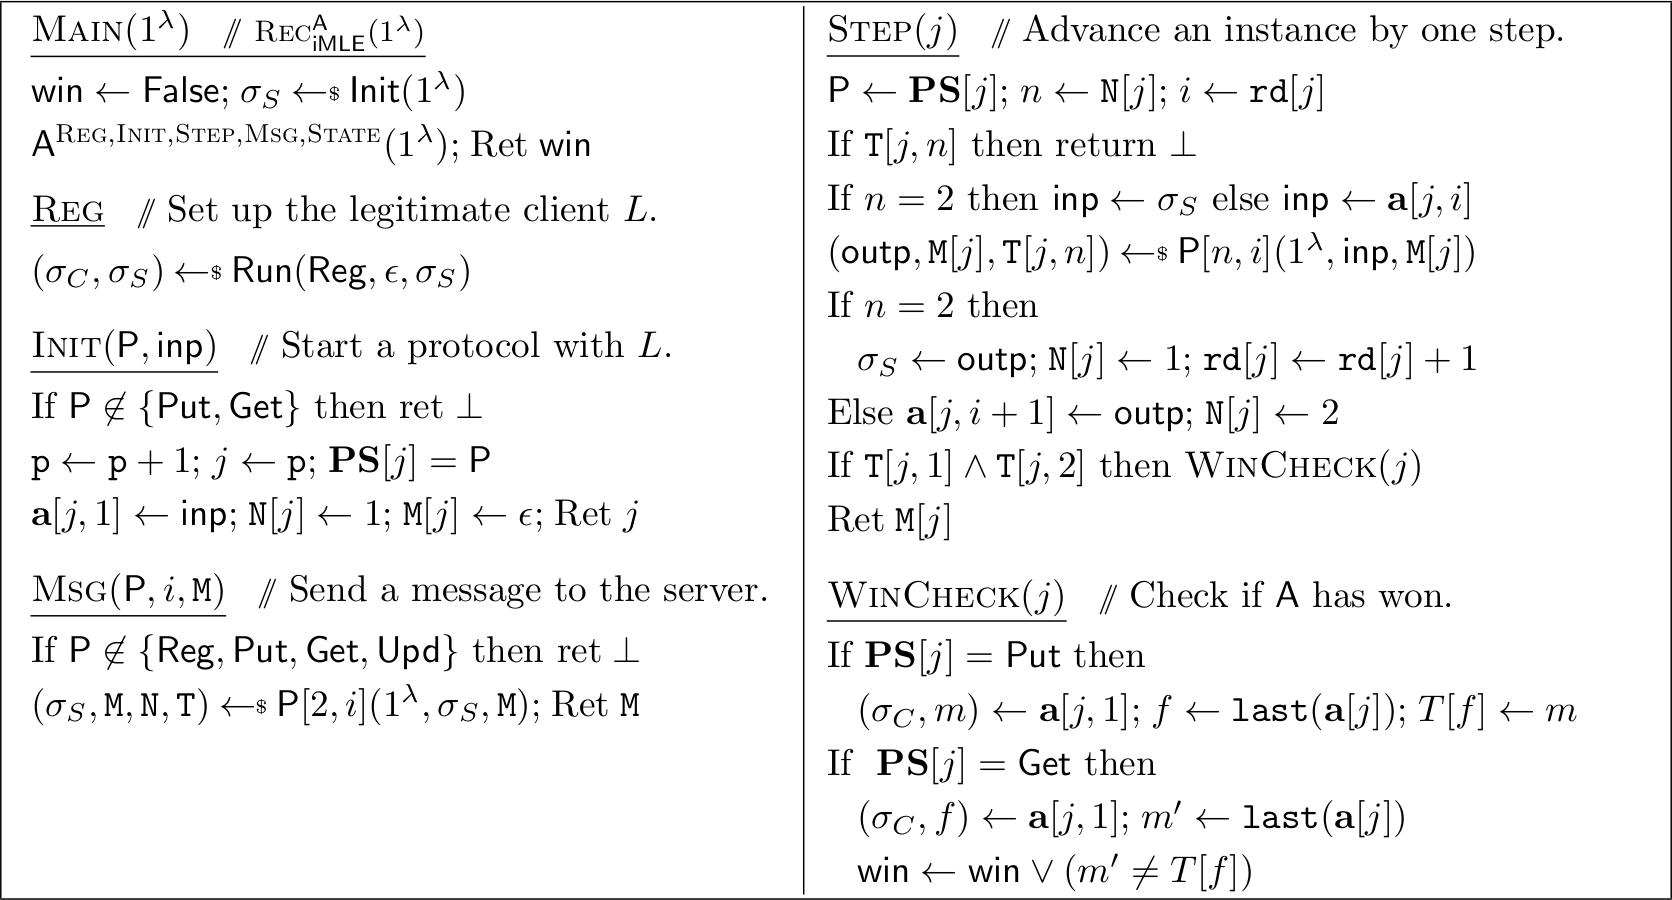
\includegraphics[width=\textwidth]{REC}
	\caption{The recovery correctness game - REC \cite{imle}}
	\label{fig:REC}
\end{figure}

	\section{Security}
	\label{subsec:security}
	The primary requirement for any secure deduplication scheme is security for unpredictable data. If the distribution from which the plaintext comes does not have negligible guessing probabability, then security cannot be achieved.\\ \\
	Privacy for unpredictable messages is captured by the \textsc{Priv} game. Unpredictability is formalized using the following notion of a source.
	\begin{enumerate}
		\item An algorithm called \textit{source} $\mathsf{S}$ which on inputs $\secparam$ and string $d \in \bin^*$ outputs a pair of tuples $(\smzero, \smone)$.
		\item All components of $\smzero$ and $\smone$ are unique. The length of each component is given by function $\ell : \NN \times \NN \rightarrow \NN $. $|\smzero[i]| = |\smone[i]| = \ell(\secpar, i)$. Similarly, there exists $m: \NN \rightarrow \NN $ so that $|\smzero| = |\smone|= m (\secpar)$.
		\item The guessing probability of $\mathsf{S}$ is
		\begin{equation*}
		\textbf{GP}_\mathsf{S}(\secpar) = max_{i,b,d}(\textbf{GP}(\textbf{m}_b[i]))
		\end{equation*}
		when $(\smzero, \smone) \sample \mathsf{S}(\secparam, d)$
		\item To model unpredictability, the guessing probability of the source $\mathsf{S}$ must be negligible.
	\end{enumerate}
	\textsc{Priv} game is formalized as follows.
	\begin{enumerate}
		\item Run \textsc{Init} to set up the server-side state.
		\item Run the source $S$ to get $(\textbf{m}_0, \textbf{m}_1)$. A random bit $b$ is selected and $\textbf{m}_b$ is used as messages to be put in the server.
		\item $A$ is invoked with oracle access to \textsc{Reg, Put, Step, Msg} and \textsc{State}. These oracles behave the same way as in \textsc{Rec} game, except that \textsc{Step} does not call \textsc{WinCheck}. \textsc{Put}($i$) means put plaintext $\textbf{m}_b[i]$.
	\end{enumerate}     
	

\begin{figure}[H]
	\centering
	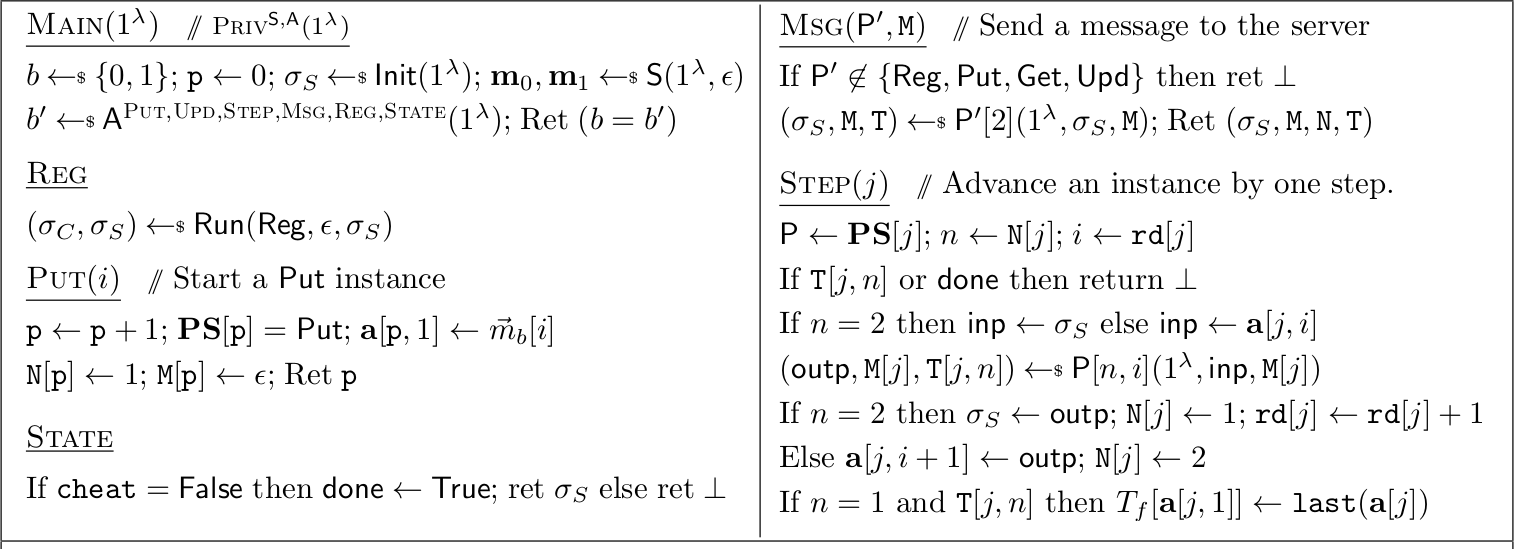
\includegraphics[width=\textwidth]{priv}
	\caption{The privacy game - PRIV \cite{imle}}
\end{figure}

	
	\section{Adversarial Model}
	The adversarial model used in this paper is similar to the one used in \cite{imle}.
	A secure deduplication system consists of a server and several clients. The attacker could control several clients simultaneously and could gain access to server storage. The adversary could also interfere the communications where he can read, relay and drop messages of legitimate clients. To simplify the protocol, we assume that the adversary cannot tamper with message contents, reorder messages within a protocol, or redirect from one protocol to another. The adversarial model captures an iMLE scheme running in the presence of an adversary with above mentioned abilities.
	\\ \\ The adversarial model is achieved by using an abstract game $G$. The games for soundness, security and other properties follow the structure similar to the one below. The objective of the game is for the adversary to violate some property of iMLE guaranteed to legitimate clients. 
	\begin{itemize}
		\item $G$ sets up and controls an instance of a server.
		\item Adversary $\adv$ is invoked with access to a set of procedures.
		\item \textsc{Msg} procedure allows adversary to set up multiple clients and to send arbitrary messages to the server.
		\item \textsc{Init} procedure starts protocol instances on behalf of a legitimate client $L$, using inputs chosen by $A$.
		\item \textsc{Step} procedure advances a  protocol instance by running the next step algorithm.
		\item \textsc{State} procedure returns the server's state - including stored ciphertexts, public parameters, etc. Only read only access is gained using this. Otherwise adversary can always tamper with the ciphertexts and win the game.
	\end{itemize}